% ─── Slide: Loss landscape — why α=0.5 is the sweet spot ─────────────────────
\begin{frame}[shrink=20]{Loss Landscape: Why $\alpha{=}0.5$ Is the Sweet Spot}
  \begin{columns}[T]
    \begin{column}{0.48\textwidth}
      \textbf{Dual-forward mixing loss:}
      \[
        \mathcal{L} = (1{-}\alpha)\,\mathcal{L}_\mathrm{FP} \;+\; \alpha\,\mathcal{L}_\mathrm{ADC}
      \]
      \begin{itemize}
        \item $\alpha{=}0$: clean FP loss only $\Rightarrow$ flat no-ADC, wide ADC gap
        \item $\alpha{=}1$: full ADC loss $\Rightarrow$ transforms over-specialise for noise,
              no-ADC PPL degrades sharply
        \item $\alpha{=}0.5$: smooth, wide minimum in both $\mathcal{L}_\mathrm{no\,ADC}$
              and $\mathcal{L}_\mathrm{ADC}$
      \end{itemize}

      \vspace{0.15em}
      \textbf{Visualisation (Li et al.\ "Filter Normalisation" method):}
      \begin{enumerate}
        \item Train FlatQuant to convergence at $\alpha \in \{0, 0.5, 1\}$
        \item Perturb $\theta^* + a\mathbf{d}_1 + b\mathbf{d}_2$
              (filter-normalised random directions)
        \item Plot $\adcppl(a,b)$ as a 2D surface / heatmap
        \item Compare sharpness of minima across $\alpha$
      \end{enumerate}

      \begin{exampleblock}{Expected result}
        $\alpha{=}0.5$ should show the widest, flattest minimum —
        both FP and ADC loss curvature are moderate.
      \end{exampleblock}
    \end{column}
    \begin{column}{0.48\textwidth}
      % plot_loss_landscape_alpha.pdf
      \iffalse
        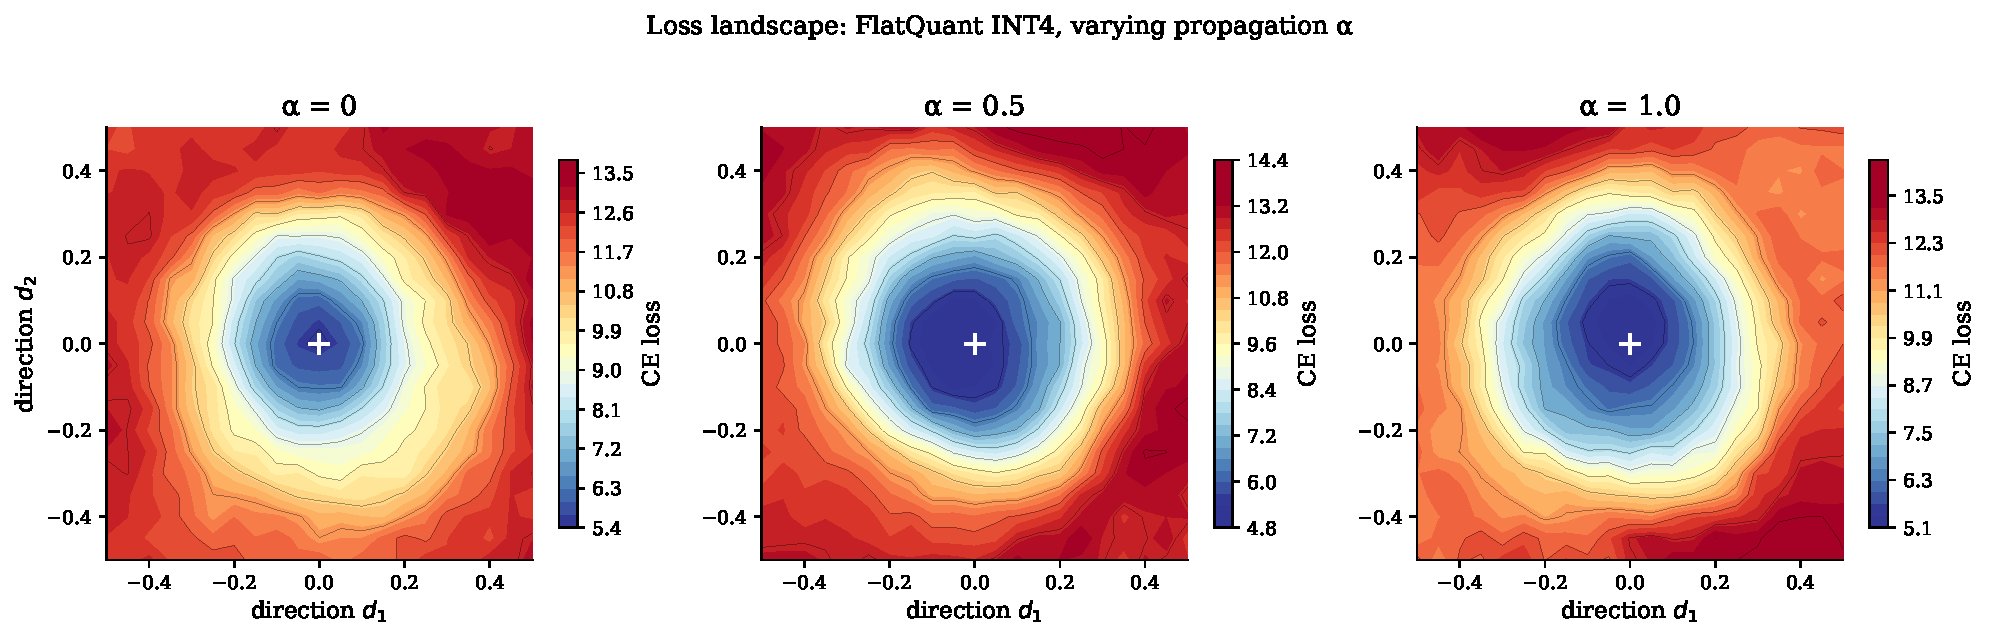
\includegraphics[width=\linewidth]{figs/plot_loss_landscape_alpha.pdf}
      \else
        \figplaceholder[0.35\textheight]{3 panels (one per $\alpha$): 2D contour heatmap of
          ADC PPL as a function of perturbation $(a, b)$ around $\theta^*$.
          Color: low PPL = blue (flat/wide), high PPL = red (sharp).
          Panel 1 ($\alpha{=}0$): narrow deep valley in no-ADC axis, flat in ADC dim.
          Panel 2 ($\alpha{=}0.5$): wide flat basin in both dims.
          Panel 3 ($\alpha{=}1$): very sharp minimum (overfit to ADC noise).
          See \texttt{experiments/loss\_landscape.md} for run instructions.}
      \fi
    \end{column}
  \end{columns}
\end{frame}
